%!TEX root = skripsi.tex
%-----------------------------------------------------------------------------%
\chapter{\babLima}
%-----------------------------------------------------------------------------%
Bab ini menjelaskan mengenai hasil yang didapatkan dari eksperimen, serta evaluasi dan analisis terkait hasil tersebut.

%-----------------------------------------------------------------------------%
\section{\textit{Sense Tagged Corpus} Bahasa Inggris}
Tabel \ref{table:sense-tagged-corpus} menunjukan jumlah token (kata) pada korpus bahasa Inggris dan yang diberikan \textit{tag sense} oleh IMS

\begin{table}
	\centering
	\caption{Jumlah \textit{instance} korpus bahasa Inggris}
	\label{table:sense-tagged-corpus}
	\begin{tabular}{|p{0.7cm}|p{4cm}|p{4cm}|}
		\hline
		No & Tipe & Jumlah
		\\ \hline
		1    & 
		Token (kata)   & 
		1.801.484
		\\ \hline
		2    & 
		Kata yang diberikan \textit{tag} oleh IMS     & 
		1.024.797 
		\\ \hline
	\end{tabular}
\end{table}

Berdasarkan proses pembuatan dan hasil dari \textit{sense tagged corpus} tersebut, dapat dilihat bahwa tidak semua kata diberikan \textit{sense} oleh IMS. Kata-kata sapaan seperti "I", "you", dan kata \textit{articles} yaitu "a", "the", "an". Tingkat kebenaran dari \textit{sense tag} yang diberikan bergantung dari model yang digunakan pada penelitian. Terdapat banyak kasus-kasus dimana pemberian \textit{sense} yang dilakukan adalah benar seperti misalnya pada kata "\textit{visitor}" yang diberikan \textit{tag} dengan \textit{sense key} 1:18:00::, yang mana berdasarkan wordnet Princeton "visitor\%1:18:00::" memiliki arti sebagai "\textit{someone who visits}". Contoh lain dari kata yang diberikan \textit{tag} dengan benar adalah "\textit{company}" pada konteks potongan kalimat "\textit{Plantation company PT ...}". Kata "\textit{company}" tersebut diberikan tag "company\%1:14:01::" yang berdasarkan wordnet Princeton memiliki makna "\textit{an institution created to conduct business}". Namun demikian, terjadinya kesalahan pemberian \textit{tag} pada kata terjadi pada kasus-kasus seperti: 

\begin{enumerate}
	\item Sebuah entitas diberikan \textit{tag} dimana entitas tersebut dianggap kata biasa. Contohnya adalah kata "Scotland Yard" dimana "Yard" pada kata tersebut diberikan \textit{tag} yang diartikan sebagai "\textit{a unit of length equal to 3 feet}". Hal ini menunjukan bahwa \textit{tool} belum dapat membedakan antara entitas yang memang tidak perlu diberikan \textit{tag} dan kata biasa (walaupun kata tersebut sudah memiliki huruf kapital).
	
	
	\item Kesalahan \textit{tag} dikarenakan \textit{training data} yang digunakan oleh model. Pada potongan kalimat "\textit{... FASB rule will cover such financial instruments as interest rate swaps financial ...}, kata "\textit{interest}" diberikan tag dengan makan "a sense of concern with and curiosity about someone or something". Berdasarkan konteks kalimat tersebut, dapat diketahui bahwa makna yang seharusnya didapat untuk kata "\textit{interest}" di atas ialah "bunga bank". Percobaan untuk \textit{tagging} sense dari kalimat "bank interest is high" juga menghasilkan \textit{sense key} yang sama untuk kata \textit{interest} (mendapatkan \textit{sense key "keingintahuan"}) walaupun pada kalimat tersebut makna yang seharusnya didapat adalah "bunga bank".
		
	\item Pemberian \textit{tag} pada \textit{multi word} token seperti "\textit{make up}" masih diberikan pada setiap kata ("\textit{make}" dan "\textit{up}" memiliki \textit{sense key} masing-masing). Hal ini terjadi karena IMS mengolah kata demi kata dengan proses tokenisasi \textit{by default} menggunakan spasi. Setelah dilakukan pemeriksaan pada kata-kata yang terdapat pada model, kata \textit{make up} ternyata disimpan sebagai "make\_up". Berdasarkan pemeriksaan tersebut, dapat disimpulkan bahwa IMS dapat melakukan \textit{tagging} yang benar dari kata "make up" jika dijadikan satu buah token berupa "make\_up". hasil \textit{tagging} yang benar untuk kasus seperti kata-kata tersebut memerlukan \textit{pre-processing} untuk mengganti \textit{separator} kata multiword yang umumnya menggunakan spasi dengan "\_" agar IMS dapat memberikan \textit{tag multi word} tersebut dengan benar. Selain \textit{pre-processing},  IMS juga dapat melakukan \textit{tagging} dengan input dalam format XML. Bentuk kata-kata dan kalimat dalam format XML tersebut biasanya memiliki \textit{multi word} yang sudah dijadikan satu token sehingga mempermudah penyelesaian masalah tersebut.
\end{enumerate}
%-----------------------------------------------------------------------------%

%-----------------------------------------------------------------------------%
\section{\textit{Word Alignment}}

Proses alignment dilakukan terhadap semua pasangan kalimat pada korpus identik (total sebanyak 88.919 buah). Hasil dari proses \textit{word alignment} yang dilakukan Giza dibandingkan dengan hasil \textit{alignment} yang dibuat oleh dua orang anotator. Jumlah yang akan dibandingkan adalah 200 buah pasangan data yang didapat dengan \textit{random sampling}. Indikator performa dari perbandingan tersebut adalah nilai dari \textit{precision}, \textit{recall}, dan F-score sesuai dengan penyesuaian cara perhitungan dari penelitian \citep{mihalcea2003evaluation}. Hasil evaluasi yang didapatkan dapat dilihat pada tabel \ref{table:word-alignment-evaluation}

\begin{table}
	\centering
	\caption{Evaluasi Word Alignment}
	\label{table:word-alignment-evaluation}
	\begin{tabular}{|p{2cm}|p{2cm}|p{2cm}|p{2cm}|}
		\hline
		Anotator & Precision & Recall & F-Score
		\\ \hline
		1 & 0.775 & 0.747 & 0.761
		\\ \hline
		2 & 0.768 & 0.75 & 0.759
		\\ \hline
	\end{tabular} 
\end{table}

\textit{Agreement} antara kedua anotator tersebut adalah 0.924. Berdasarkan hasil tersebut, dapat dilihat bahwa Giza++ secara umum dapat menghasilkan \textit{alignment} cukup baik untuk korpus identik yang digunakan. Namun demikian, kesalahan ataupun kelemahan yang sering terjadi dari \textit{alignment} Giza adalah pada kasus-kasus seperti:

\begin{enumerate}
	\item Pemasangan frasa kompleks dengan kata lain. Seperti misalnya frasa "\textit{a very awesome and huge building}" dengan "gedung raksasa", ataupun gaya bahasa lainnya yang menjadikan frasa tersebut kompleks dan panjang.
	\item Pasangan kalimat yang tidak sepenuhnya paralel (\textit{comparable}), seperti misalnya "I'm glad that you're here" dengan "Aku senang kau ada". Variasi dari bentuk kalimat \textit{comparable} terkadang mempersulit model dari Giza++ untuk menentukan pasangan kata yang benar.
\end{enumerate}

Walaupun akurasi yang didapatkan sekitar 70\%, tidak jarang ditemukan pasangan kata-kata yang tidak sesuai dan dapat menjadi masalah pada saat \textit{sense transfering} sehingga dilakukan proses \textit{word alignment enhancement}.

Hasil \textit{enhancement} dengan pendekatan \textit{bi-directional} masih menghasilkan kata-kata yang memiliki pasangan tidak sesuai seperti misalnya kata "pembuat" dengan "\textit{jewelry}", kata "pendidikan" dengan "\textit{tended}", kata "harapkan" dengan "\textit{anticipate}", dan lain-lain. Skenario pada \textit{enhancement} menggunakan \textit{crawling} kamus Indonesia-Inggris tidak menghasilkan pasangan yang salah seperti pada contoh yang diberikan di atas. Evaluasi terhadap hasil \textit{enhancement} ini dilakukan dengan mengambil 10 buah \textit{sample} secara \textit{random} dari pasangan kata yang ada. Hasil \textit{sampling} tersebut dapat dilihat pada \ref{table:random-sampling-enhancement}.

\begin{table}
	\centering
	\caption{Pasangan kata hasil \textit{random sampling} dengan pendekatan \textit{bi-directional} dan \textit{crawling}}
	\label{table:random-sampling-enhancement}
	\begin{tabular}{|p{4cm}|p{4cm}|p{4cm}|}
		\hline
		\textbf{Kata} & \textbf{\textit{Bi-directional}} & \textbf{\textit{Crawling}}
		\\ \hline
		memodernkan & \textit{modernize} & \textit{modernize} \\ \hline
		kembar & \textit{twin}, \textit{twins} & \textit{twin}, \textit{twins} \\ \hline
		ingat & \textit{remember}, \textit{remembered}, \textit{recall}, \textit{note}, \textit{recalls}, \textit{strike} & \textit{remembered}, \textit{recall}, \textit{remember} \\ \hline
		peroksida & peroxide & peroxide \\ \hline
		imbang & \textit{draw}, \textit{drawing} & \textit{draw}, \textit{drawing} \\ \hline
		tegang & \textit{tense}, \textit{edge} & \textit{tense} \\ \hline
		berobat & \textit{medical}, \textit{purpose}, \textit{treatment} & \textit{treatment} \\ \hline
		membantu & \textit{bolster}, \textit{supporting}, \textit{beneficial}, \textit{helping}, \textit{help}, \textit{support}, \textit{assisted}, \textit{assist}, \textit{appearance}, \textit{assisting}, \textit{helped}, \textit{assists}, \textit{helps}, \textit{aiding}, \textit{aid}, \textit{facilitates}, \textit{supports}, \textit{assistance} & \textit{helped}, \textit{assisting}, \textit{facilitating}, \textit{help}, \textit{assisted}, \textit{assist}, \textit{helpful}, \textit{helping}, \textit{helps}, \textit{aid}, \textit{facilitates}, \textit{supports}, \textit{avail} \\ \hline
		disusun & \textit{composed}, \textit{arranged}, \textit{developed}, \textit{structured}, \textit{organized}, \textit{prepared}, \textit{compiled} & \textit{composed}, \textit{arranged}, \textit{developed}, \textit{structured}, \textit{prepared}, \textit{compiled} \\ \hline
		diusulkan & \textit{suggested}, \textit{suggests}, \textit{recommended}, \textit{proposed}, \textit{proposes} & \textit{suggested}, \textit{proposed} \\ \hline
	\end{tabular}
\end{table}

Pasangan kata pada tabel di atas kemudian dihitung berapa jumlah pasangan yang benar untuk masing-masing pendekatan (\textit{bi-directional} dan \textit{crawling}). Pasangan kata dianggap benar jika hasil translasi kata tersebut dapat digunakan untuk konteks kalimat tertentu. Hasil evaluasi dengan mengukur precision dari hasil tersebut dapat dilihat pada tabel \ref{table:enhancement-precision}.


\begin{table}
	\centering
	\caption{Precision dari hasil \textit{random sampling alignment enhancement}}
	\label{table:enhancement-precision}
	\begin{tabular}{|p{2.5cm}|p{3cm}|p{3cm}|}
		\hline
		Kata & \textbf{\textit{Bi-directional}} & \textbf{\textit{Crawling}}
		\\ \hline
		memodernkan & 1.0 & 1.0 \\ \hline
		kembar & 1.0 & 1.0 \\ \hline
		ingat & 0.67 & 1.0 \\ \hline
		peroksida & 1.0 & 1.0 \\ \hline
		imbang & 0.5 & 0.5 \\ \hline
		tegang & 1.0 & 1.0 \\ \hline
		berobat & 0.33 & 1.0 \\ \hline
		membantu & 0.73 & 0.84 \\ \hline
		disusun & 0.71 & 0.66 \\ \hline
		diusulkan & 0.6 & 1.0 \\ \hline	
		\hline
		\textbf{Rata-rata} & 0.78 & 0.90 \\ \hline
	\end{tabular}
\end{table}

Berdasarkan evaluasi pada tabel di atas, didapatkan bahwa pendekatan \textit{crawling} pada \textit{random sampling} tersebut memiliki tingkat precision yang lebih tinggi dari \textit{bi-directional} yaitu sebesar 90\%. Kamus hasil dari \textit{crawling} inilah yang akan digunakan untuk proses \textit{sense transfering}.

%-----------------------------------------------------------------------------%
\section{\textit{Sense Transfering}}

Proses \textit{transfer} makna kata dari bahasa Inggris ke bahasa Indonesia yang dilakukan sangat bergantung dari hasil \textit{alignment} kata pada proses sebelumnya. Untuk sebagian besar kata yang memiliki pasangan kata yang benar, proses \textit{transfer} dapat menghasilkan makna yang benar juga. Hal tersebut didukung jika \textit{sense tagged word} pada korpus bahasa Inggris juga benar). Terdapat beberapa kata yang dipilih sebagai \textit{sampling} untuk mengevaluasi hasil \textit{sense transfering}. Kelompok ini dibagi menjadi:

\begin{enumerate}
	\item Jumlah Kelas
	\begin{enumerate}
		\item 3-5 kelas kata
		\item lebih dari 5 kelas kata
	\end{enumerate}
	\item sebaran jumlah \textit{instance} dalam kelasnya
	\begin{enumerate}
		\item \textit{balance}
		\item \textit{imbalance}
	\end{enumerate}
	\item Bentuk morfologi dari kata tersebut
	\begin{enumerate}
		\item Lemma (kata dasar)
		\item Berimbuhan baik itu infleksional ataupun \textit{derivative}
	\end{enumerate}
\end{enumerate}

Pada laporan ini, hasil dari \textit{sense transfering} yang dianalisis adalah proses yang menggunakan kamus \textit{crawling}. Pada jumlah kelas sebanyak 3-5 kelas kata (\textit{sense key}), \textit{target word} yang diambil adalah "memecahkan". Kata tersebut memiliki 4 buah kelas total dengan \textit{sense key} yang didapat yaitu 'solve\%2:31:00::','resolve\%2:31:01::', 'break\%2:30:03::', dan 'split\%2:38:00::'. Kata "menolak" mewakili kelas kata sebanyak 9 buah yang diantaranya mengandung kelas 'reject\%2:40:00::', 'decline\%2:32:00::', rebuff\%2:32:00::, dan enam buah kelas lainnya. Makna kata 'decline\%2:32:00::' sendiri sebenarnya merupakan "gabungan" dengan 'refuse\%2:32:00' yang memiliki kemiripan dengan nilai \textit{path similarity} melewati batas \textit{threshold}, sehingga makna kata dianggap sama dan diberikan \textit{tag} sebagai 'decline' (dipilih satu \textit{tag} saja). Tabel \ref{table:number-classes-sense-transfering-evaluation} menunjukan contoh beberapa kata tersebut dalam beberapa konteks kalimat yang bersesuaian.

\begin{table}
	\centering
	\caption{Evaluasi \textit{Sense Transfering} Berdasarkan Jumlah Kelas}
	\label{table:number-classes-sense-transfering-evaluation}
	\begin{tabular}{|p{4cm}|p{4cm}|p{4cm}|}
		\hline
		\textit{Sense Key} & Makna & Kalimat
		\\ \hline
		solve\%2:31:00::  & 
		\textit{find the solution to (a problem or question) or understand the meaning of}   & 
		salah satu cara untuk \textbf{memecahkan} persoalan yang pelik...
		\\ \hline
		resolve\%2:31:01:: & 
		\textit{bring to an end / settle conclusively}   & 
		evolusionis masih belum bisa \textbf{memecahkan} permasalahan darwin...
		\\ \hline
		break\%2:30:03:: & 
		\textit{terminate}   & 
		...base mereka \textbf{memecahkan} rekor untuk...
		\\ \hline
		split\%2:38:00:: &
		\textit{go one's own way; move apart;} &
		senat mereka \textbf{memecahkan} perbedaan antara skenario 1 dan 3 dengan
		\\ \hline
		decline\%2:32:00:: &
		\textit{show unwillingness towards} &
		wells rich \textbf{menolak} untuk berkomentar...
		\\ \hline
		rebuff\%2:32:00:: &
		\textit{reject outright and bluntly} &
		georgia gulf \textbf{menolak} penawaran tersebut ...
		\\ \hline
		reject\%2:40:00:: &
		\textit{refuse to accept} &
		..dua pekan lalu \textbf{menolak} tawaran pemerintah...
		\\ \hline
	\end{tabular}
\end{table}

Makna kata \textit{split} yang diberikan hanya berjumlah satu buah dari keseluruhan korpus, hal ini disebabkan karena kata bahasa Inggris yang digunakan pada kalimat bahasa Inggrisnya menggunakan kata \textit{split}. Berdasarkan \textit{sampling} yang dilakukan, jumlah kelas kata yang ada bergantung pada sebanyak apa sebuah kata di bahasa Indonesia dipasangkan dengan kata bahasa Inggris yang berbeda dan memiliki makna pada \textit{sense tagged english corpus}. Jumlah kelas ini dapat bergantung pada seberapa akurasi \textit{alignment} kata yang dilakukan pada proses sebelumnya.

Pada sebaran jumlah \textit{instance} di dalam kelas-kelasnya, kata "kehadiran" memiliki jumlah kelas \textit{attendance} (19 buah), \textit{presence} (64 buah), dan \textit{existence
} 1 buah. Perbandingan kedua kelas dengan \textit{instance} terbanyak tersebut adalah 19:64 yaitu 0.29. Kedua \textit{sense} tersebut memiliki makna yang kurang lebih menyatakan sebuah \textit{state} dimana seseorang datang/hadir. Sementara itu, kelas kata "rumahnya" memiliki jumlah \textit{instance} sebanyak 32 buah pada kelas "house", dan 19 buah pada kelas "home". Perbandingan kedua kelas pada kata "rumahnya" tersebut adalah 0.59, yang mana rasio tersebut yang lebih besar dari rasio kelas kata "kehadiran" (0.29). Tabel \ref{table:class-instance-sense-transfering-evaluation} menunjukan makna kata yang dipindahkan berdasarkan \textit{sampling} berdasarkan sebaran \textit{instance} dalam kelas.

\begin{table}
	\centering
	\caption{Evaluasi \textit{Sense Transfering} Berdasarkan Sebaran Kelas}
	\label{table:class-instance-sense-transfering-evaluation}
	\begin{tabular}{|p{4cm}|p{2.85cm}|p{2.85cm}|p{1.2cm}|}
		\hline
		Kata (Sense key) & Makna & Kalimat & Jumlah
		\\ \hline
		Kehadiran (attendance\%1:04:00::)  & 
		\textit{the act of being present (at a meeting or event etc.)}   & 
		...tingkat \textbf{kehadiran} guru di sekolah... &
		19
		\\ \hline
		Kehadiran (presence\%1:09:00::) & 
		\textit{the impression that something is present}   & 
		...berkurangnya \textbf{kehadiran} pria dewasa...
		&
		64
		\\ \hline
		rumahnya (house\%1:14:02::) & 
		\textit{an official assembly having legislative powers} & 
		...kebakaran yang melanda \textbf{rumahnya}...
		& 32
		\\ \hline
		rumahnya (home\%1:06:00::) &
		\textit{Housing that someone is living in} &
		...ia pulang ke \textbf{rumahnya} pada sabtu...
		& 19
		\\ \hline
	\end{tabular}
\end{table}

Kedua makna pada kata "kehadiran" memiliki makna yang relatif dekat dan sesuai dalam konteks kalimat kata tersebut muncul. Namun demikian, \textit{sense key} pada kata rumah yaitu "house\%1:14:02::" memiliki makna yang salah, dimana sense key yang lebih tepat semestinya adalah house\%1:06:01:: dengan makna "\textit{a building in which something is sheltered or located}". Kesalahan makna kata yang dipindahkan tersebut disebabkan karena kata \textit{house} pada korpus inggris diberikan tag 'house\%1:14:02::'. Kesalahan ini seperti yang sudah dijelaskan pada analisis \textit{tagging} IMS pada sub-bab Pembuatan \textit{Sense Tagged Corpus} Bahasa Inggris.


Kelompok \textit{sampling} lain adalah makna yang akan dilihat pada kata dengan bentuk morfologi yang berbeda. Kata "makan", "makanan", dan "memakan" merupakan kata yang mewakili kasus bentuk morfologi dalam bentuk lemma maupun berimbuhan. Pada kata "makan", \textit{sense key} yang diterima dari hasil \textit{transfer} adalah eat\%2:34:00:: yang memiliki makna "\textit{take in solid food}". Kata "makanan" pada kalimat-kalimat yang ada diberikan \textit{sense key} food\%1:03:00:: yang diartikan sebagai "\textit{any substance that can be metabolized by an animal to give energy and build tissue}". Kata "memakan" sendiri memiliki beberapa \textit{sense key} seperti consume\%2:34:02::, eat\%2:34:00::, dan feed\%1:13:00::. Dari \textit{sense key} yang didapat tersebut, consume\%2:34:02::("spend extravagantly") bukan merupakan \textit{sense} yang tepat (seharusnya memiliki makna mengonsumsi makanan), dan feed\%1:13:00:: ("\textit{food for domestic livestock}") yang semestinya adalah "memberikan makanan".

Terdapat beberapa kata-kata yang dipilih secara manual untuk dihitung akurasi dari kesesuaian \textit{tag} makna yang didapat. Kriteria pemilihan kata-kata sebagai \textit{sample} ini yaitu memiliki pasangan kata  dalam Bahasa Inggris dan makna kata lebih dari satu. Evaluasi ini akan menghitung seberapa banyak kelas-kelas makna kata yang benar dari hasil \textit{transfering} pada kata-kata pilihan tersebut. Hasil akurasi dari jumlah makna kata yang tepat dapat dilihat pada tabel \ref{table:akuras-kelas-makna-kata}.

\begin{longtable}{|p{1.8cm}|p{1.2cm}|p{5cm}|p{1.2cm}|p{1.5cm}|} 
	\hline
	Kata & Jumlah \textit{sense key} & \textit{sense key}  & Jumlah \textit{sense key} yang benar & Akurasi \\ \hline
	halaman & 3 &  page\%1:10:00::, yard\%1:23:00::, courtyard\%1:06:00:: & 2 & 0.67 \\ \hline
	coklat & 3 & cocoa\%1:13:02, cacao\%1:20:00::, brown\%5:00:00:chromatic:00 & 3 & 1.0 \\ \hline
	debu & 2 & dust\%1:27:00::, plume\%1:06:00:: & 1 & 0.5 \\ \hline
	batasan & 7 & limit\%1:07:00::, restriction\%1:09:00::, restraint\%1:04:00::, limitation\%1:23:00::, definition\%1:10:00::, constraint\%1:26:00::, limit\%2:30:01:: & 5 & 0.71 \\ \hline
	lingkungan & 7 & environment\%1:26:00::, environmental\%3:01:01::, neighborhood\%1:14:00::, environmentally\%4:02:00::, sphere\%1:15:00::, surroundings\%1:15:00::, outside\%5:00:00:external:00 & 5 & 0.71 \\ \hline
	hakim & 3 & judge\%1:18:01::, justice\%1:04:00::, magistrate\%1:18:00:: & 2 & 0.67 \\ \hline
	hati & 3 & heart\%1:09:00::, liver\%1:08:00::, mind\%1:09:00:: & 2 & 0.67 \\ \hline
	memecah-kan & 4 & solve\%2:31:00::, resolve\%2:31:01::, break\%2:30:03::, split\%2:38:00:: & 3 & 0.75 \\ \hline
	\caption{Evaluasi \textit{sense transfering} akurasi kelas makna kata}
	\label{table:akuras-kelas-makna-kata}
\end{longtable}
 
Berdasarkan tabel di atas, rerata akurasi yang didapatkan pada kata-kata tersebut adalah 0.73. Terdapat beberapa makna hasil \textit{transfer} yang tidak sesuai dengan kata pasangannya seperti misalnya "plume\%1:06:00::" dengan kata "debu" yang memiliki makna "\textit{a feather or cluster of feathers worn as an ornament}, atau \textit{sense key} "limit\%2:30:01::" dengan makna "\textit{place limits on (extent or access)}" pada kata "batasan". \textit{Sense key} "limit\%2:30:01::" tersebut dianggap tidak sesuai dengan kata "batasan" karena makna yang dikandung adalah "memberi batas" dan bukan "batasan" itu sendiri.

Pada hasil tabel tersebut, dipilih beberapa kata-kata yang ambigu (memiliki makna kata yang tidak mirip) secara manual untuk dievaluasi pada tahap berikutnya. Pada tahap ini, evaluasi dilakukan anotator dengan menghitung berapa jumlah makna hasil \textit{transfer} pada kata tersebut, yang sesuai dengan kalimat dimana kata itu muncul. Makna kata yang tidak sesuai dari hasil evaluasi sebelumnya tidak dimasukkan ke dalam proses ini. Hasil evaluasi dapat dilihat pada tabel \ref{table:evaluasi-sense-transfer-2}.

\begin{table}
	\centering
	\caption{Evaluasi \textit{sense transfering} berdasarkan jumlah kesesuaian dengan kalimat}
	\label{table:evaluasi-sense-transfer-2}
	\begin{tabular}{|p{4cm}|p{2.85cm}|p{2.85cm}|p{1.2cm}|}
		\hline
		Kata dan \textit{sense key} & Jumlah benar & Jumlah kalimat & Akurasi
		\\ \hline
		halaman (page\%1:10:00::) & 29 & 41 & 0.70 \\ \hline
		halaman (courtyard\%1:06:00::) & 3 & 3 & 1.0 \\ \hline
		coklat (cocoa\%1:13:02::) & 6 & 10 & 0.6 \\ \hline
		coklat (brown\%5:00:00:chro-matic:00) & 3 & 4 & 0.75 \\ \hline
		coklat (cacao\%1:20:00::) & 4 & 5 & 0.8 \\ \hline
		hati (heart\%1:09:00::) & 166 & 170 & 0.97 \\ \hline
		hati (liver\%1:08:00::) & 44 & 44 & 1.0 \\ \hline
		memecahkan (solve\%2:31:00::) & 12 & 13 & 0.92 \\ \hline
		memecahkan (resolve\%2:31:01::) &  & 7 & \\ \hline
		memecahkan (split\%2:38:00::) & 1 & 1 & 1.0 \\ \hline
	\end{tabular}
\end{table}

Pada tabel di atas, didapatkan hasil dari rerata akurasi kesesuaian makna kata hasil \textit{transfering} dengan kalimat sebesar <INSERTAKURASIHERE>. Ketidaksesuaian sense "page\%1:10:00::" (halaman buku) pada kata "halaman", terjadi pada kalimat yang mengandung makna "halaman \textit{web}" dan bukan halaman buku. Kesalahan pada kata "hati" juga disebabkan karena "\textit{heart}" diberikan \textit{tag} "hati (perasaan)" dan pada beberapa kasus, "\textit{heart}" yang dimaksud adalah "\textit{heart} (jantung)".
 
Berdasarkan berbagai hasil evaluasi di atas, makna kata yang tidak tepat merupakan kesalahan dari baik itu variasi \textit{alignment} suatu kata yang dipasangkan dengan kata lainnya, ataupun juga hasil \textit{tagging} model IMS yang yang tidak tepat. Pada kesalahan hasil \textit{alignment} kasus yang terjadi adalah ketika suatu kata dipasangkan dengan kata lain yang tidak tepat sehingga berpengaruh pada makna kata yang dipindahkan. Kesalahan \textit{tagging} pada IMS juga mengakibatkan kesalahan \textit{sense key} pada kata Bahasa Indonesia karena pada \textit{sense tagged corpus} sudah mengalami kesalahan.
%-----------------------------------------------------------------------------%
\section{WSD Bahasa Indonesia}

Untuk melihat seberapa baik performa sistem WSD dengan menggunakan \textit{sense tagged corpus} hasil dari penelitian, terdapat kata-kata yang dipilih secara manual sebagai sampling dari \textit{target word} yang akan dievaluasi berdasarkan nilai F-score dari hasil rata-rata \textit{cross validation}. Kata yang dipilih merupakan \textit{instance} yang memiliki pasangan kata lebih dari satu dalam bahasa Inggris dan mempunyai makna yang berbeda dari hasil \textit{sense transfering}. \textit{Target word} yang dipilih tersebut memiliki kriteria bahwa pasangan bahasa inggris kata tersebut lebih dari satu ataupun juga pasangan bahasa inggrisnya memiliki makna yang tidak dekat (ambigu). Fitur yang dilakukan percobaan pada penelitian ini adalah F1(\textit{bag of words}), F2 (\textit{word embedding}), F3 (\textit{pos-tag}), F4 (\textit{pos tagging} dan \textit{bag of words}). Hasil evaluasi dapat dilihat pada tabel akurasi  \ref{table:wsd-evaluation-crawling} berikut.
\begin{table}
	\centering
	\caption{Evaluasi sistem WSD}
	\label{table:wsd-evaluation-crawling}
	\begin{tabular}{|p{3cm}|p{1.5cm}|p{1.5cm}|p{1.5cm}|p{1.5cm}|p{1.5cm}|}
		\hline
		Kata & Baseline & F1 & F2 & F3 & F4 \\ \hline
		memecahkan & 0.5 & 0.51 & 0.62 & 0.48 & 0.51 \\ \hline
		menolak & 0.6 & 0.63 & 0.6 & 0.76 & 0.74 \\ \hline
		obat & 0.49 & 0.58 & 0.62 & 0.56 & 0.63 \\ \hline
		lingkungan & 0.54 & 0.51 & 0.42 & 0.7 & 0.66 \\ \hline
		halaman & 0.93 & 0.9 & 0.88 & 0.83 & 0.88 \\ \hline
		kehadiran & 0.67 & 0.93 & 0.8 & 0.72 & 0.88 \\ \hline
		hati & 0.72 & 0.88 & 0.82 & 0.75 & 0.89 \\ \hline
		coklat & 0.33 & 0.61 & 0.48 & 0.34 & 0.67 \\ \hline
		berat & 0.53 & 0.5 & 0.46 & 0.64 & 0.66 \\ \hline
		jalan & 0.66 & 0.72 & 0.74 & 0.69 & 0.72 \\ \hline
	\end{tabular} 
\end{table}


\begin{comment}

\begin{table}
	\centering
	\caption{Evaluasi sistem WSD kamus \textit{bi-directional}}
	\label{table:wsd-evaluation-bidirectional}
	\begin{tabular}{|p{3cm}|p{1.5cm}|p{1.5cm}|p{1.5cm}|p{1.5cm}|p{1.5cm}|}
		\hline
		Kata & Baseline & f1 & f2 & f3 & f4 \\ \hline
		memecahkan & 0.46 & 0.46 & 0.46 & 0.38 & 0.42 \\ \hline
		menolak & 0.63 & 0.65 & 0.57 & 0.75 & 0.76 \\ \hline
		obat & 0.5 & 0.58 & 0.54 & 0.45 & 0.55 \\ \hline
		lingkungan & 0.55 & 0.55 & 0.45 & 0.67 & 0.68 \\ \hline
		halaman & 0.85 & 0.9 & 0.85 & 0.77 & 0.88 \\ \hline
		kehadiran & 0.68 & 0.85 & 0.75 & 0.67 & 0.81 \\ \hline
		hati & 0.75 & 0.86 & 0.85 & 0.75 & 0.86 \\ \hline
		coklat & 0.17 & 0.72 & 0.5 & 0.33 & 0.67 \\ \hline
		berat & 0.49 & 0.63 & 0.52 & 0.68 & 0.68 \\ \hline
		jalan & 0.68 & 0.76 & 0.71 & 0.71 & 0.76 \\ \hline
	\end{tabular} 
\end{table}

\end{comment}

Pada hasil akurasi (F-Score) tabel tersebut, dapat terlihat bahwa pada fitur F1, tujuh dari sepuluh (70\%) buah kata memiliki nilai performa di atas baseline, tujuh dari sepuluh kata (70\%) mengungguli baseline pada fitur F2, delapan dari sepuluh kata (80\%) mengungguli baseline pada fitur F3, dan sembilan dari sepuluh kata (90\%) mengungguli baseline pada fitur F4. Rerata performa dari hasil tersebut dapat dilihat pada tabel \ref{table:performa-rerata-wsd}.

\begin{table}
	\centering
	\caption{Performa rerata sistem WSD Bahasa Indonesia}
	\label{table:performa-rerata-wsd}
	\begin{tabular}{|p{2cm}|p{2cm}|p{2cm}|p{2cm}|p{2cm}|}
		\hline
		Baseline & F1 & F2 & F3 & F4 \\ \hline
		%0.62 & 0.710 & 0.646 & 0.651 & 0.716 \\ \hline
		0.597 & 0.677 & 0.644 & 0.647 & 0.724 \\ \hline
	\end{tabular}
\end{table}

Berdasarkan rata-rata dari nilai F-Score tersebut, dapat dilihat bahwa untuk kesepuluh data \textit{sampling} yang digunakan, rerata dari F-Score semua fitur mengungguli sistem baseline.

Grafik perbandingan dari fitur-fitur tersebut untuk setiap kata dapat dilihat pada gambar \ref{fig:fitur-wsd-indo}.

\begin{figure}[H]
	\begin{subfigure}{.5\textwidth}
		\centering
		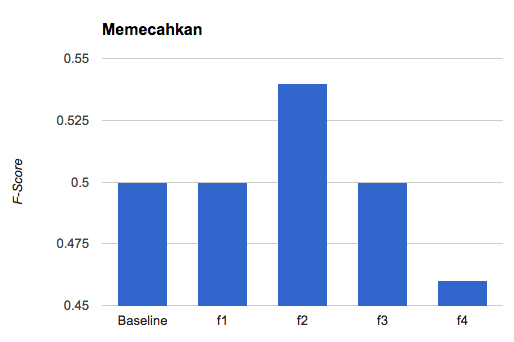
\includegraphics[width=1\linewidth]{adit_pics/memecahkan.png}
		\caption{memecahkan}
	\end{subfigure}%
	\begin{subfigure}{.5\textwidth}
		\centering
		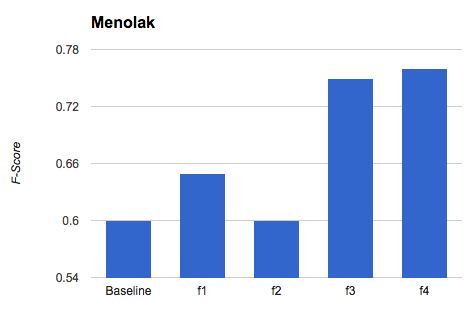
\includegraphics[width=1\linewidth]{adit_pics/menolak.png}
		\caption{menolak}
	\end{subfigure}%
	\\
	\begin{subfigure}{.5\textwidth}
		\centering
		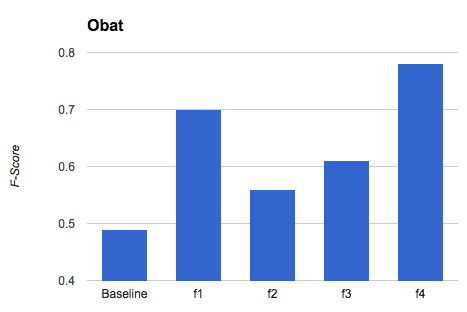
\includegraphics[width=1\linewidth]{adit_pics/obat.png}
		\caption{obat}
	\end{subfigure}%
	\begin{subfigure}{.5\textwidth}
		\centering
		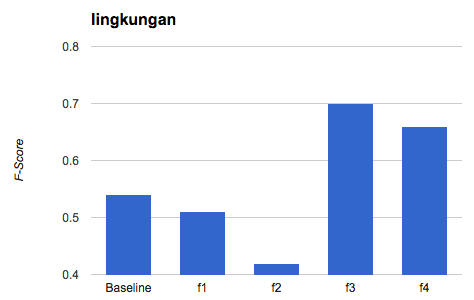
\includegraphics[width=1\linewidth]{adit_pics/lingkungan.png}
		\caption{lingkungan}
	\end{subfigure}%
	\\
	\begin{subfigure}{.5\textwidth}
		\centering
		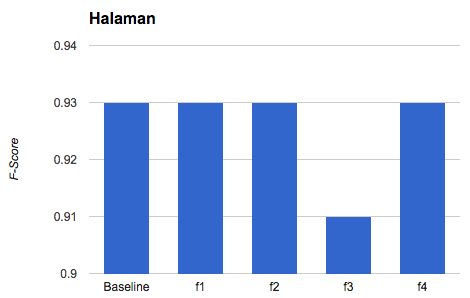
\includegraphics[width=1\linewidth]{adit_pics/halaman.png}
		\caption{halaman}
	\end{subfigure}%
	\begin{subfigure}{.5\textwidth}
		\centering
		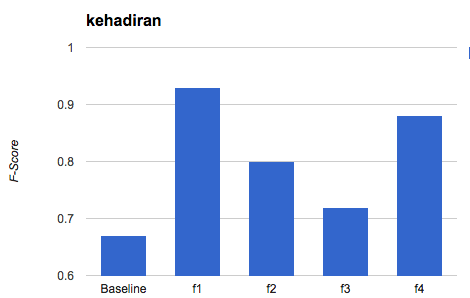
\includegraphics[width=1\linewidth]{adit_pics/kehadiran.png}
		\caption{kehadiran}
	\end{subfigure}%
	\\
	\begin{subfigure}{.5\textwidth}
		\centering
		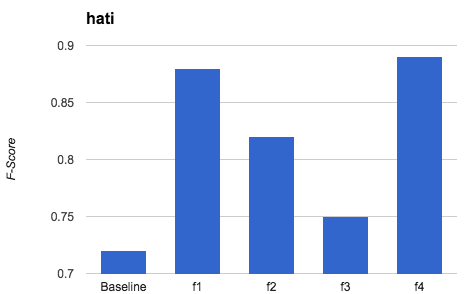
\includegraphics[width=1\linewidth]{adit_pics/hati.png}
		\caption{hati}
	\end{subfigure}%
	\begin{subfigure}{.5\textwidth}
		\centering
		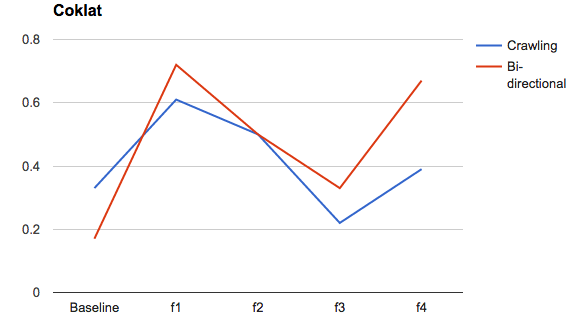
\includegraphics[width=1\linewidth]{adit_pics/coklat.png}
		\caption{coklat}
	\end{subfigure}%
\end{figure}
\clearpage	
\begin{figure}[H]
	\ContinuedFloat
	\begin{subfigure}{.5\textwidth}
		\centering
		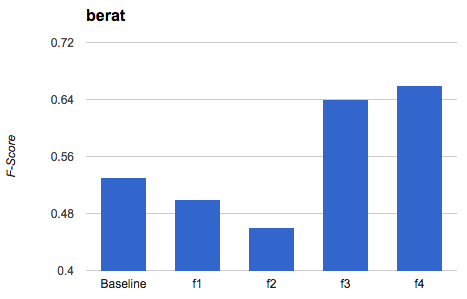
\includegraphics[width=1\linewidth]{adit_pics/berat.png}
		\caption{berat}
	\end{subfigure}%
	\begin{subfigure}{.5\textwidth}
		\centering
		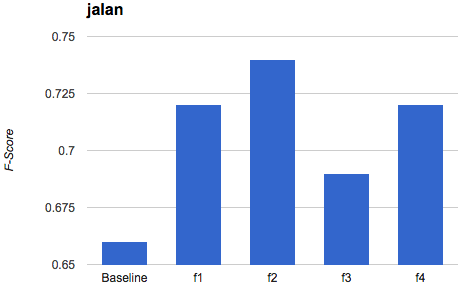
\includegraphics[width=1\linewidth]{adit_pics/jalan.png}
		\caption{jalan}
	\end{subfigure}%
	\caption{Grafik Performa Fitur WSD Bahasa Indonesia}
	\label{fig:fitur-wsd-indo}
\end{figure} 

Berdasarkan sepuluh grafik di atas, dapat kita lihat bahwa sembilan dari sepuluh \textit{sample} kata yang dicoba, hanya satu kata yang tidak pernah memiliki performa lebih baik baseline yaitu kata "halaman". Sembilan kata lainnya selalu memiliki performa di atas baseline untuk minimal satu dari keempat fitur yang dicoba. Pada tujuh buah \textit{sample}, fitur F2 memiliki akurasi di bawah F1 walaupun sudah menggunakan \textit{word embedding}. Pada lima buah \textit{sample} kata, F4 yang merupakan fitur gabungan F1 dan F3 memiliki performa yang lebih baik dari fitur F1 saja. Penggunaan berbagai skenario fitur tersebut menunjukan bahwa fitur F1 atau F4 memiliki performa minimal sama atau di atas baseline pada sembilan dari sepuluh \textit{sample} (90\%), hal ini menunjukkan bahwa \textit{bag of words} ataupun kombinasinya dengan POS Tag dapat mengungguli baseline pada \textit{sampling} ini. Jumlah persentase pada \textit{sampling} dengan fitur F2 yang mengungguli baseline adalah 70\%. Performa F2 yang lebih rendah dari F4 pada rerata F-Score dapat disebabkan karena domain yang berbeda antara \textit{training data} pada saat membentuk model \textit{word embedding} (perbedaan pada gaya bahasa pada Wikipedia dan korpus identik). Namun demikian, persentase terbesar dari \textit{sampling} sepuluh kata di atas diperoleh pada fitur F4 yang memiliki performa lebih baik dari baseline pada sembilan kasus dari sepuluh kata tersebut (90\%).